
\section{Laplace-Transformation}
	$$\boxed{f(t) \; \laplace \; F(s)=\int\limits_0^\infty f(t)e^{-st}dt} \qquad \boxed{ s=\sigma+j\omega}$$\\
	\begin{tabular}{p{0.5cm}p{17.5cm}}
		$\bullet$ & Definitionsbereich nur für kausale Systeme $t\geq 0$\\
		%$\bullet$ & Integrierbar über das Intervall $(0,\infty)$\\
		$\bullet$ & Wachstum kleiner als der von einer Exponentialfunktion\\ 
		$\bullet$ & Gegen"uber $j\omega$ bei der Fourier-Transformation ist bei der
			Laplace-Transformation $s$ verallgemeinert zu $s=\sigma + j\omega$. Das
			bedeutet, dass die Fourier-Transformierte $F(j\omega)$ durch die
			Laplace-Transformation $F(s)$ ausgedr\"uckt werden kann. \\
		$\bullet$ & mit 
		$\begin{cases} 
		\sigma = 0 & \rightarrow \text{Amplitude bleibt konstant} \\ 
		\sigma > 0 & \rightarrow \text{explodiert die Amplitude f\"ur } 0 < t \rightarrow \infty \\
		\sigma < 0 & \rightarrow \text{klingt die Amplidute für } 0 < t \rightarrow \infty \text{ auf $0$ ab} \
		 \end{cases} $ \\   
	\end{tabular}
	
 	\subsection{Eigenschaften der Laplace-Transformation}
  		\renewcommand{\arraystretch}{2}
		\begin{tabular}{|ll|}
	        \hline
	        	Linearität & 
	 			$\alpha\cdot f(t) + \beta\cdot g(t) \; \laplace \; \alpha\cdot F(s) + \beta\cdot
	 			G(s)$ \\
			\hline
	 			"Ahnlichkeit / Streckung im Zeitbereich &
	 			$f(\alpha t) \; \laplace \; \frac{1}{\alpha}F \left (\frac{s}{\alpha} \right ) \quad 0 <\alpha, \alpha \in\mathbb{R}$ \\
	 		\hline
	 		\hline
	 			Faltung im Zeitbereich &
	 			$f(t) \ast g(t) = \int\limits_{0}^{t} f(\tau)g(t-\tau)d\tau \; \laplace \; F(s)
	 			\cdot G(s)$\\
	 		\hline
	 			Faltung im Frequenzbereich &
	 			$f(t) \cdot g(t) \; \laplace \; \frac{1}{2\pi j}\int\limits_{c-j\infty}^{c+j\infty}
	 			F(\xi) G(s-\xi)d\xi$ \\
	 		\hline
	 		\hline
	 			1te Ableitung im Zeitbereich &
	 			$\frac{\partial f(t)}{\partial t} \; \laplace \; sF(s)
	 			-f(0^+)$ \\
	 		\hline
	 			2te Ableitung im Zeitbereich &
	 			$\frac{\partial f(t)}{\partial t} \; \laplace \; s^2F(s)
	 			-sf(0^+) -f'(0^+)$ \\
	 		\hline
	 			nte Ableitung im Zeitbereich &
	 			$\frac{\partial^n f(t)}{\partial t^n} \; \laplace \; s^nF(s)
	 			-s^{n-1}f(0^+)-s^{n-2}\frac{\partial f(0^+)}{\partial t}-\ldots
	 			-s^0\frac{\partial^{n-1} f(0^+)}{\partial t^{n-1}}$ \\
	 		\hline
	 			Ableitung im Frequenzbereich &
		 		$(-t)^n f(t) \; \laplace \;  \frac{\partial^n F(s)}{\partial s^n}$ \\
	 		\hline
	 		\hline
	 			Verschiebung im Zeitbereich nach rechts &
	 			$\sigma(t-a)f(t - a) \; \laplace \; F(s)*e^{-as}$ \\
	 		\hline
				Verschiebung im Zeitbereich nach links &
				$\sigma(t-a)f(t + a) \; \laplace \; e^{as} \cdot [F(s) - \int\limits_0^{a} f(t) \cdot e^{-st} dt]$\\
			\hline
	 			Verschiebung im Frequenzbereich (Dämpfungssatz) &
	 			$f(t)e^{\pm\alpha t} \; \laplace \; F(s\mp\alpha)$ \\
	 		\hline
	 		\hline
	 			Integration im Originalbereich (Sprungantwort)&
	 			$\int\limits_0^t f(u)du \; \laplace \; \frac{1}{s}\cdot F(s)$ \\
	 		\hline
	 			Multiplikation mit $t$ &
	 			$t\cdot f(t)  \; \laplace \; \frac{-\partial F(s)}{\partial s}$ \\
 			\hline
 			\hline
	 			Anfangswert &
	 			$\lim_{t\rightarrow 0^+} f(t) = \lim_{s\rightarrow \infty} sF(s),\text{~wenn
	 			}  \lim_{t\rightarrow 0} f(t)\text{~existiert}.$ \\
 			\hline
	 			Endwert &
	 			$\lim_{t\rightarrow \infty} f(t) = \lim_{s\rightarrow 0} sF(s),\text{~wenn
	 			}  \lim_{t\rightarrow \infty} f(t)\text{~existiert}.$ \\
	 		\hline
       	\end{tabular}
		\renewcommand{\arraystretch}{\arraystretchOriginal}
		
		
		%TODO Dies ist ein Beispiel, wie man die Laplace-Tabelle gestalten könnte
%		\begin{tabular}{|l|l|ll|}
%			\hline
%			\multicolumn{3}{|l}{Linearität}   & asdf \\ \hline
%			\multirow{4}{*}{Ableitung} & \multirow{3}{*}{Zeitbereich} & 1te & asdf \\ \cline{3-4} 
%			&  & 2te  &  asdf\\ \cline{3-4}
%			&  & nte  &  asdf\\ \cline{2-4} 
%			& \multicolumn{2}{l}{Frequenzbereich} & asdf\\ \hline
%		\end{tabular}
		
		
		
		
		
		
	
	\subsection{Laplace-Tabelle}
	\renewcommand{\arraystretch}{2}
	\hrule
	\begin{minipage}{9cm}
		\begin{center}
			\begin{tabular}{p{4cm}p{0.75cm}p{3cm}}
				$\sigma \left( t \right)$ & $\; \laplace \;$ & $\dfrac{1}{s}$ \\
				
				$\sigma \left( t \right) \cdot t$ & $\; \laplace \;$ & $\dfrac{1}{s^2}$\\
				
				$\sigma \left( t \right) \cdot t^2$ & $\; \laplace \;$ & $\dfrac{2}{s^3}$\\
				
				$\sigma \left( t \right) \cdot t^n$ & $\; \laplace \;$ & $\dfrac{n!}{s^{n+1}}$\\
				
				$\sigma \left( t \right) \cdot e^{\alpha t}$ & $\; \laplace \;$ &
				$\dfrac{1}{s-\alpha}$\\
				
				$\sigma \left( t \right) \cdot t \cdot e^{\alpha t}$ & $\; \laplace \;$ & $\dfrac{1}{( s - \alpha )^2}$\\
				
				$\sigma \left( t \right)\cdot t^2 \cdot e^{\alpha t}$ &
				$\; \laplace \;$ & $\dfrac{2}{{( s - \alpha )}^3}$\\
				
				$\sigma \left( t \right)\cdot t^n \cdot e^{ \alpha t}$ &
				$\; \laplace \;$ & $\dfrac{n!}{(s-\alpha)^{n+1}}$\\
				
				$\sigma \left( t \right)\cdot \dfrac { 1 - e ^ { - \alpha t } } { \alpha }$ & $\; \laplace \;$ & $\dfrac { 1 } { s ( s + \alpha ) }$\\
				
				$\sigma \left( t \right)\cdot \dfrac {e ^ { - \alpha t }+\alpha t -1 } { \alpha^2 }$ & $\; \laplace \;$ & $\dfrac { 1 } { s^2 ( s + \alpha ) }$\\
				
				$\sigma \left( t \right)\cdot \dfrac {1- e ^ { - \alpha t } - \alpha t e ^ {- \alpha t }}{ \alpha ^2 }$ & $\; \laplace \;$ & $\dfrac { 1 } { s ( s + \alpha )^2 }$\\
					
			\end{tabular}
		\end{center}
	\end{minipage}
\vline
\begin{minipage}{9cm}
\begin{center}
	\begin{tabular}{p{5cm}p{0.75cm}p{3cm}}
	
		$\delta \left( t \right)$ & $\; \laplace \;$ & $1\left( s \right)$ \\
		
		$\delta \left( t - \alpha \right)$ & $\; \laplace \;$ & $e^{- \alpha s}$\\
		
		$\sigma\left( t - \alpha \right)$ & $\; \laplace \;$ & $ \dfrac{1}{s} \cdot e^{- \alpha s}$\\
		
		$\sigma \left( t \right) \cdot \sin \left(\omega t \right)$ & $\; \laplace \;$ &
		$\dfrac{\omega}{s^2 + {\omega^2}}$\\
		
		$\sigma \left( t \right) \cdot \cos \left( \omega t \right)$ & $\; \laplace \;$ &
		$\dfrac{s}{ s^2 + \omega^2}$\\
		
		$\sigma \left( t \right) \cdot  e^{ \alpha t} \cdot \sin \left(\omega t \right)$ & $\; \laplace \;$ 
		& 	$\dfrac{\omega}{(s-a)^2 + {\omega^2}}$\\
		$\sigma \left( t \right) \cdot e^{ \alpha t} \cdot \cos \left( \omega t \right) $ & $\; \laplace \;$ &
		$\dfrac{s-a}{(s-a)^2 + \omega^2}$\\
		
		$\sigma \left( t \right)\cdot t \cdot \dfrac{\sin \left( \alpha t \right)} { 2 \alpha }$ & $\; \laplace \;$ & $\dfrac{s}{ \left(s^ {2}+ \alpha ^{2} \right)^{2}}$ \\
		
		$\sigma \left( t \right)\cdot \dfrac { e ^ { - \alpha t } - e ^ { - \beta t } } { \beta - \alpha }$ & $\; \laplace \;$ & $\dfrac { 1 } { ( s + \alpha ) ( s + \beta ) }$\\
		
		$\sigma \left( t \right)\cdot \dfrac {(\alpha - \beta) +\beta e ^ { - \alpha t } - \alpha e ^ { - \beta t } } { \alpha \beta (\alpha - \beta) }$ & $\; \laplace \;$ & $\dfrac { 1 } {s ( s + \alpha ) ( s + \beta ) }$\\
		
		$\sigma \left( t \right)\cdot \dfrac { e ^ { - \beta t } ( \alpha \cos ( \alpha t ) - \beta \sin ( \alpha t ) ) } { \alpha }$& $\; \laplace \;$ & $\dfrac { s } { ( s + \beta ) ^ { 2 } + \alpha ^ { 2 } }$\\
		
		 
		
		
	\end{tabular}
\end{center}
\end{minipage}


\newpage
\renewcommand{\arraystretch}{\arraystretchOriginal}		
	\subsection{Rücktransformation}
		\subsubsection{Vorgehen}
				1. Kürzen oder vereinfachen \\
				2. Partialbruchzerlegung falls nötig \\
				3. Rücktransformation mittels Laplace-Tabelle \\
				4. $h(t)\hspace{0.2cm}\underline{nicht} < 0$ \\
			
		\subsubsection{Residuensatz}
			Beispiel:\\
			$F(s) = \frac{1}{(s+\alpha)(s+\beta)}, \qquad (0 < \alpha,\beta \in \mathbf{R}, \alpha \neq \beta)$\\
			$f(t) = \frac{1}{2\pi j} \int\limits_{-j\infty}^{j\infty} F(s)e^{st} ds = \sum\limits_{i=1}^k Res(F(s_k)e^{s_kt})$\\
			$=\lim_{s \to -\alpha} ((s+\alpha)F(s)e^{st}) + \lim_{s \to -\beta}((s+\beta)F(s)e^{st})$\\
			$=\frac{e^{-\alpha t}}{\beta - \alpha} + \frac{e^{-\beta t}}{\alpha - \beta} = \frac{e^{-\alpha t}-e^{-\beta t}}{\beta - \alpha}$
			
			
	\subsection{Lösung linearer Differentialgleichungen}
		\begin{minipage}{11.5cm}
			\renewcommand{\arraystretch}{2}
			\begin{tabular}{| l | l |}
				\hline
					Übertragungsfunktion & $G(s) = \frac{1}{p(s)}$\\
					& $g(t) \; \laplace \; G(s)$ \\
				\hline
					Frequenzgang & $G(j\omega) = H(\omega)$ \\
				\hline
					Impulsantwort & $y_{\delta}(t) = g(t) = y_{\sigma}'(t) \; \laplace \; G(s) = \frac{1}{p(s)}=Y_{\delta}(s)$\\
				\hline
					Sprungwantwort & $y_{\sigma}(t)=\int\limits_0^t g(u) du \; \laplace \; \frac{G(s)}{s} = \frac{1}{s \cdot p(s)} = Y_{\sigma}(s)$\\
				\hline
					Eigenschwingung & $\frac{h(s)}{p(s)}$ \\
				\hline
					äussere Erregung & $\frac{F(s)}{p(s)}$ \\
				\hline
					stationärer Zustand & = ungedämpfte Eigenschwingung\\
				\hline
			\end{tabular}
			\renewcommand{\arraystretch}{\arraystretchOriginal}\\
		\end{minipage}
		\begin{minipage}{8cm}
					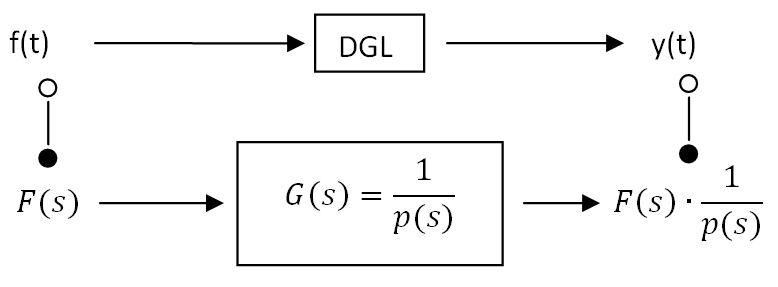
\includegraphics[width=8cm]{./bilder/diffgleichungen2.png} \\
		\end{minipage}
		
		
		\begin{minipage}[l]{16cm}
				\textbf{Beispiel:} $y'' + 8y' + 25y = \sigma{t} \cdot \sin(2t)$ mit $y(0) = 2, y'(0) = -1$\\
				
				$\sin(2t) \; \laplace \; \frac{2}{s^2+4}$ \\ $Y(s)(s^2+8s+25) = 2s+15+\frac{2}{s^2+4}$
				$\Leftrightarrow Y(s) = \frac{2s+15}{s^2+8s+25}+\frac{2}{(s^2+4)(s^2+8s+25)}=
				\underbrace{\frac{2s+15}{s^2+8s+25}}_\text{Eigenschwinung durch Anfangszustand} +
				\underbrace{\frac{As + B}{s^2+4}}_\text{stationärer Zustand} +
				\underbrace{\frac{Cs + D}{s^2+8s+25}}_\text{Eigenschwinung durch Einschalten}$
		\end{minipage}
		\subsubsection{Eigenschwingungen}
			Aus der Eigenschwingung können die Nullstellen des charakteristischen Polynom $p(s)$ 
			direkt abgelesen werden. \\
			\textbf{Beispiel:} \\
			$y(t) = \frac{1}{2} e^{-t} \sin(3t) - \frac{2}{3} e^{-2t} \cos(2t) = 
			\underbrace{\frac{1}{2} e^{\textcolor{red}{-t}} \frac{1}{2j}(e^{\textcolor{red}{3j}t}
			-e^{\textcolor{red}{-3j}t})}_{NS = EW = \textcolor{red}{-1 \pm 3j}} - 
			\underbrace{\frac{2}{3} e^{\textcolor{red}{-2}t} \frac{1}{2}(e^{\textcolor{red}{2j}t}
			+e^{\textcolor{red}{-2j}t})}_{NS = EW = \textcolor{red}{-2 \pm 2j}}$ \\\\
			Damit ist das char. Polynom $p(s) = (s-NS_1)(s-NS_2)\ldots(s-NS_n)$ \\
			Bei mehreren gemessenen Eigenschwingungen werden die char. Polynome multipliziert. \\
			Der stationäre Zustand ist $\lim\limits_{t\rightarrow\infty}y(t) = \frac{1}{p(0)}$ *(Endwertsatz) \\
				
		
	\subsection{Eigenschwingung}
		\begin{minipage}{12cm}
			Spezielle Anfangswerte bei einem System ohne äussere Einflüsse:\\
			$y(0) = 0, y'(0) = 0, \dots , y^{(n-2)} = 0, y^{(n-1)} = 1$\\
			in diesem Fall wird $h(s) = 1$\\
		\end{minipage}
		\begin{minipage}{6cm}
			\begin{math}
				\begin{aligned}
					y(t) \; &\laplace \; Y(s)\\
					y'(t) \; &\laplace \; sY(s) - y_0\\
					y''(t)\; &\laplace \; s^2Y(s) - sy_0 - y'_0\\ 
					y'''(t)\; &\laplace \; s^3Y(s) - s^2y_0 - sy'_0 - y''_0\\ 
					\vdots&\\
					y^{(n)} \; &\laplace \; 
					\underbrace{s^nY(s)}_{Y(s) \cdot p(s)}
					\underbrace{-s^{n-1}y_0 - \dots - y^{(n-1)}}_{h(s)}
				\end{aligned}
			\end{math}
		\end{minipage}